\chapter{Struktur af rapporten}\label{chap:struktur-af-problemanalyse}

I dette kapitel, beskrives strukturen af rapporten. Strukturen er baseret på beskrivelsen af et
informationssystem fra \citet{Laudon1999}. Komponenterne i et informationssystem er illustreret i
\myref{fig:kontekstmodel}.

\begin{figure}[htbp]
  \centering
  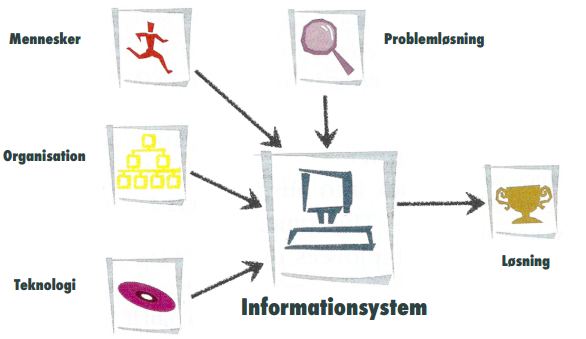
\includegraphics{images/kontekstmodel/metode.png}
  \caption[Metode for Kontekstmodellen]{Illustration af elementerne i et informationssystem. Kilde:
  \protect\citet{Laudon1999}}
  \label{fig:kontekstmodel}
\end{figure}


\section{Informationssystem}\label{Informationssystem}

Et informationssystem bruges til at effektivisere en arbejdsproces og hjælper med at holde fokus, så arbejdet
bliver gjort tilfredsstillende. Informationssystemet består af tre processor: indsamling af data, behandling
af dataene og formidling af dataene. Der indsamles data om de tre elementer: mennesker, organisation og
teknologi. Når dataene er indsamlet, behandles de, altså der bliver analyseret på dataene. Herefter formidles
det i form af der findes ud af hvad datene kan bruges til. Behandlingen af de tre elementer bruges til at
finde ud af, hvad der skal tages hensyn til under problemløsningsdelen. Alt dette er et informationssystem,
som bruges til finde ud af, hvad løsningen til problemstillingen er.


\subsection{Mennesker}\label{subsec:mennesker}

Elementet mennesker handler om personer/persongrupper, som har en interesse i, at en given problemstilling
løses. Det kan være brugeren af det program, der bliver lavet og andre som får gavn af en løsning. Man
undersøger bl.a. brugerens evner, da programmet skal laves på en sådan måde, at brugeren har den
fornødne kunnen, til at kunne betjene programmet. Brugerens behov undersøges også, så man får alle de funktioner
med, som er nødvendige for at programmet er brugbart.


\subsection{Organisation}\label{subsec:organisation}

Under organisationsafsnittet undersøges hvor og hvordan problemet opstår, derudover undersøges der hvilke regler
og værdier organisationen har, for at kunne tage disse med til problemløsningen.


\subsection{Teknologi}\label{subsec:Teknologi}

Teknologielementet handler om teknologier som allerede er på markedet, som kan løse problemstillingen. Dette
behøver ikke kun at være løsninger som er computerbaserede, det kan også være manuelle systemer, altså hvor
det hele gøres i hånden, med papir og blyant.


\section{Rapportens opbygning}\label{sec:rapportens-opbygning}

Først bliver menneskedelen behandlet, i form af en interessentanalyse, herefter vil organisationselementet blive berørt. Derefter bliver der skrevet om teknologier,
hvorefter de tre elementer munder ud i en problemafgrænsning og en problemformulering. Til sidst skrives der
om problemløsningsdelen. \fxnote{Sidste sætning skal udvides så der står hvad der vil blive skrevet om}
